%----------------------------------------------------------------------------------------
%	PACKAGES AND OTHER DOCUMENT CONFIGURATIONS
%----------------------------------------------------------------------------------------

\documentclass[final]{beamer}

\usepackage[scale=1.24]{beamerposter} % Use the beamerposter package for laying out the poster
\usepackage{subcaption}
\usepackage{float}
\usetheme{confposter} % Use the confposter theme supplied with this template

\setbeamercolor{block title}{fg=ngreen,bg=white} % Colors of the block titles
\setbeamercolor{block body}{fg=black,bg=white} % Colors of the body of blocks
\setbeamercolor{block alerted title}{fg=white,bg=dblue!70} % Colors of the highlighted block titles
\setbeamercolor{block alerted body}{fg=black,bg=dblue!10} % Colors of the body of highlighted blocks
% Many more colors are available for use in beamerthemeconfposter.sty

%-----------------------------------------------------------
% Define the column widths and overall poster size
% To set effective sepwid, onecolwid and twocolwid values, first choose how many columns you want and how much separation you want between columns
% In this template, the separation width chosen is 0.024 of the paper width and a 4-column layout
% onecolwid should therefore be (1-(# of columns+1)*sepwid)/# of columns e.g. (1-(4+1)*0.024)/4 = 0.22
% Set twocolwid to be (2*onecolwid)+sepwid = 0.464
% Set threecolwid to be (3*onecolwid)+2*sepwid = 0.708

\newlength{\sepwid}
\newlength{\onecolwid}
\newlength{\twocolwid}
\newlength{\threecolwid}
\setlength{\paperwidth}{48in} % A0 width: 46.8in
\setlength{\paperheight}{36in} % A0 height: 33.1in
\setlength{\sepwid}{0.024\paperwidth} % Separation width (white space) between columns
\setlength{\onecolwid}{0.22\paperwidth} % Width of one column
\setlength{\twocolwid}{0.464\paperwidth} % Width of two columns
\setlength{\threecolwid}{0.708\paperwidth} % Width of three columns
\setlength{\topmargin}{-0.5in} % Reduce the top margin size
%-----------------------------------------------------------

\usepackage{graphicx}  % Required for including images

\usepackage{booktabs} % Top and bottom rules for tables

%----------------------------------------------------------------------------------------
%	TITLE SECTION 
%----------------------------------------------------------------------------------------

\title{CityU Car Survives Through Hong Kong} % Poster title

\author{LIU Bonan, LIU Yuzhan, PU Ziyi, TIAN Zonghang, XIE Dong} % Author(s)

\institute{Master of Science in Data Science, City University of Hong Kong} % Institution(s)

%----------------------------------------------------------------------------------------

\begin{document}

\addtobeamertemplate{block end}{}{\vspace*{2ex}} % White space under blocks
\addtobeamertemplate{block alerted end}{}{\vspace*{2ex}} % White space under highlighted (alert) blocks

\setlength{\belowcaptionskip}{2ex} % White space under figures
\setlength\belowdisplayshortskip{2ex} % White space under equations

\begin{frame}[t] % The whole poster is enclosed in one beamer frame

\begin{columns}[t] % The whole poster consists of three major columns, the second of which is split into two columns twice - the [t] option aligns each column's content to the top

\begin{column}{\sepwid}\end{column} % Empty spacer column

\begin{column}{\onecolwid} % The first column

%----------------------------------------------------------------------------------------
%	OBJECTIVES
%----------------------------------------------------------------------------------------

\begin{alertblock}{ABSTRACT} % main idea

This project first simulated the complex traffic situation in Hong Kong as the environment: narrow and sinuous roads layout, obstacles alongside, pedestrians and animals come from all the directions accidentally, besides, limited time for the commute.
A 3D back-engine supercar(named UFO) was then modeled in that environment, whose task is to drive to the target terminal point safe and as quickly as possible. \\
We control UFO through Unity ML-Agent API, deploy the Reinforcement Learning algorithm to help UFO learning to survive from random routes.

\end{alertblock}

%----------------------------------------------------------------------------------------
%	INTRODUCTION
% Background, motivation, and the main idea

% –Theory and/or Application

% –Numerical experiments

% –Conculsion + limitation & strength of the methods + possible extensions(theory & algorithm & application)
%----------------------------------------------------------------------------------------

\begin{block}{Introduction} % background and motivation
\textbf{Theory Support} Deep Reinforcement learning algorithms are commonly used in many areas, such as the famous Alpha-Go, real-time gaming, and auto driving.

\textbf{Motivation} We notice that Hong Kong faced a very complex traffic situation than many other cities, even supercities like Shenzhen or Washington. Roads here are much narrow and sinuous, and some segments are located between mountain and sea. The very high density of buildings makes it possible that pedestrians suddenly appear from any horizontal direction, not to say wild pigs and other animals.

\textbf{Our Target} We try to simulate the traffic situation of HK, and 'build' a self-driving car, deploy RL algorithms to help it driving to the target terminal point safe and as quickly as possible.

% cite demo
% This statement requires citation \cite{Smith:2012qr}.

\end{block}

% already covered this part by dividing the poster, but in report still needs one

\begin{figure}
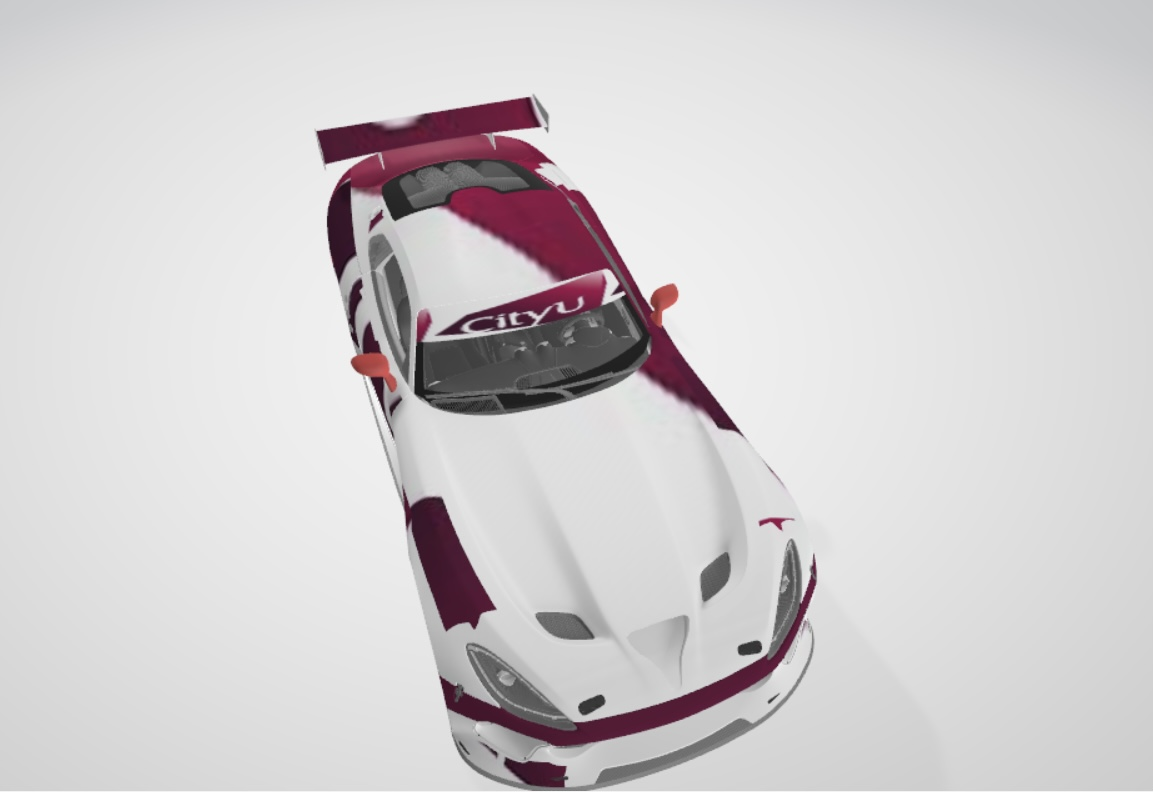
\includegraphics[width=0.6\linewidth]{carModel.jpeg}
\caption{Car Agent}
\end{figure}

\end{column} % End of the first column
%----------------------------------------------------------------------------------------


\begin{column}{\sepwid}\end{column} % Empty spacer column

\begin{column}{\twocolwid} % Begin a column which is two columns wide (column 2)

\begin{columns}[t,totalwidth=\twocolwid] % Split up the two columns wide column

\begin{column}{\onecolwid}\vspace{-.6in} % The first column within column 2 (column 2.1)

%----------------------------------------------------------------------------------------
%	MATERIALS
%----------------------------------------------------------------------------------------

\begin{block}{Unity 3D Engine} % Unity 

Unity 3D engine can be used to create three-dimensional, two-dimensional, virtual reality, and augmented reality games, as well as simulations and other experiences.\\

The Unity Machine Learning Agents Toolkit (ML-Agents) is an open-source project that enables games and simulations to serve as environments for training intelligent agents.\\

We generated random routes and obstacles' locations every time. And assigned a series of sensors(ray casting sensors, trigger collider sensors, and spherical sensors) to the car agent made it agile to drive.

\end{block}

%----------------------------------------------------------------------------------------

\end{column} % End of column 2.1

\begin{column}{\onecolwid}\vspace{-.6in} % The second column within column 2 (column 2.2)

%----------------------------------------------------------------------------------------
%	METHODS
%----------------------------------------------------------------------------------------

\begin{block}{RL Algorithm}

This project adopted Proximal Policy Optimization(PPO), which is an on-policy algorithm which can be used for environments with either discrete or continuous action spaces. This means that it explores by sampling actions according to the latest version of its stochastic policy. The amount of randomness in action selection depends on both initial conditions and the training procedure. Over the course of training, the policy typically becomes progressively less random, as the update rule encourages it to exploit rewards that it has already found. This may cause the policy to get trapped in local optima.

\end{block}

%----------------------------------------------------------------------------------------

\end{column} % End of column 2.2

\end{columns} % End of the split of column 2 - any content after this will now take up 2 columns width

%----------------------------------------------------------------------------------------
%	IMPORTANT RESULT
%----------------------------------------------------------------------------------------

\begin{alertblock}{3D Enviroment Captures}

% The Unity Machine Learning Agents Toolkit (ML-Agents) is an open-source project that enables games and simulations to serve as environments for training intelligent agents. 
\begin{figure}
    % \centering
    \begin{subfigure}[bH]{0.15\textwidth}
        % \centering
        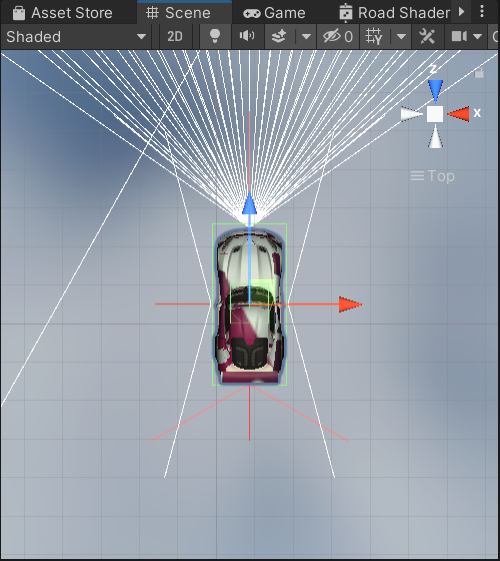
\includegraphics[width=\textwidth]{radar.PNG}
        \caption{Agent's radar}
        \label{fig:radar}
    \end{subfigure}
    \hfill
    \begin{subfigure}[bH]{0.15\textwidth}
        % \centering
        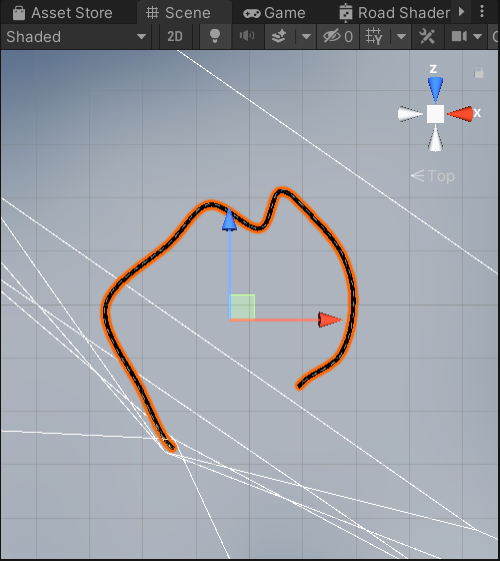
\includegraphics[width=\textwidth]{road1.PNG}
        \caption{Random route1}
        \label{fig:rr1}
    \end{subfigure}
    \hfill
    \begin{subfigure}[bH]{0.15\textwidth}
        % \centering
        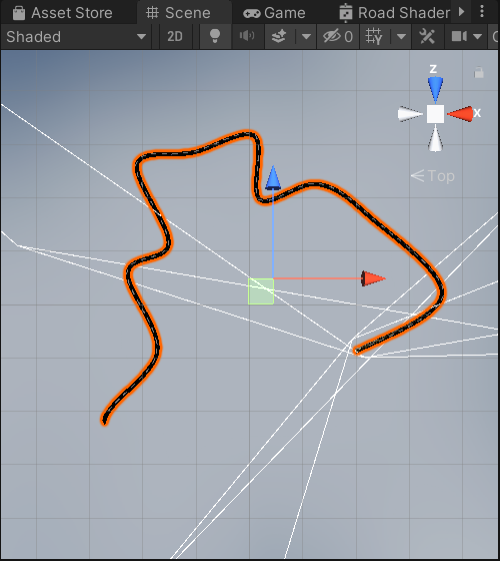
\includegraphics[width=\textwidth]{road2.PNG}
        \caption{Random route2}
        \label{fig:rr2}
    \end{subfigure}
    \hfill
    \begin{subfigure}[bH]{0.15\textwidth}
        % \centering
        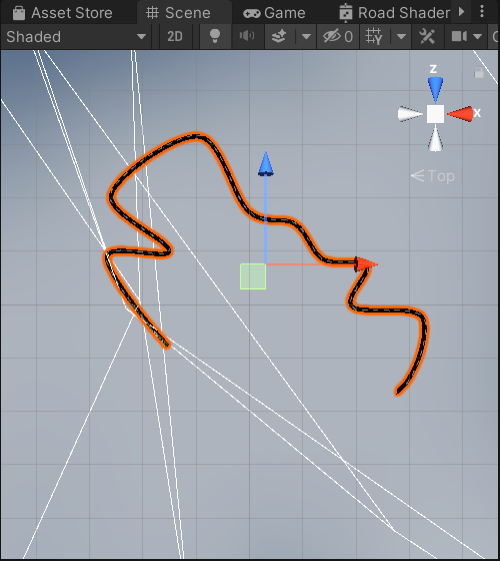
\includegraphics[width=\textwidth]{road3.PNG}
        \caption{Random route3}
        \label{fig:rr3}
    \end{subfigure}
    \hfill
    \begin{subfigure}[bH]{0.15\textwidth}
        % \centering
        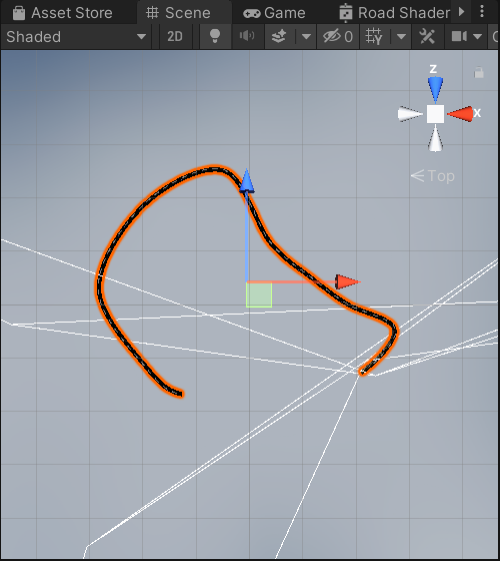
\includegraphics[width=\textwidth]{road4.PNG}
        \caption{Random route4}
        \label{fig:rr4}
    \end{subfigure}
    %    \caption{Unity Enviroment Elements}
       \label{fig:unity}
\end{figure}

\end{alertblock} 

%----------------------------------------------------------------------------------------

\begin{columns}[t,totalwidth=\twocolwid] % Split up the two columns wide column again

\begin{column}{\onecolwid} % The first column within column 2 (column 2.1)

%----------------------------------------------------------------------------------------
%	MATHEMATICAL SECTION
%----------------------------------------------------------------------------------------

\begin{block}{Experiment Setting and Launch}
The below table listed hardware and software settings during our experiment.
\begin{table}
\vspace{2ex}
\begin{tabular}{l l }
\toprule
\textbf{Item} & \textbf{Information}\\
\midrule
Memory & 32G, mini. 16G  \\
CPU & AMD/Intel 8 Core(2.6GHz-2.9GHz) \\
GPU& NVIDIA RTX 2060 (Optional)\\
Unity& Version: 2020.3.1f1 \\
ML-Agent& Version: Relese 14 \\
Pedestrians& Red light balls in Unity\\
obstacles& Static stone balls in Unity \\
Target Point& Clint('s photo) in Unity \\
\bottomrule
\end{tabular}
\caption{Experiment Setting}
\end{table}


\end{block}

%----------------------------------------------------------------------------------------

\end{column} % End of column 2.1

\begin{column}{\onecolwid} % The second column within column 2 (column 2.2)

%----------------------------------------------------------------------------------------
%	RESULTS
%----------------------------------------------------------------------------------------

\begin{block}{Results}

\begin{figure}
    % \centering
    \begin{subfigure}[b]{0.4\textwidth}
        % \centering
        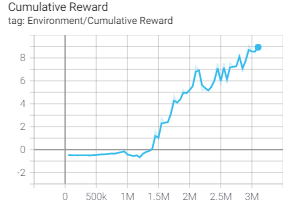
\includegraphics[width=\textwidth]{cum_reward.PNG}
        \caption{Cumulative Reward}
        \label{fig:Cum Reward}
    \end{subfigure}
    % \hfill
    \begin{subfigure}[b]{0.4\textwidth}
        % \centering
        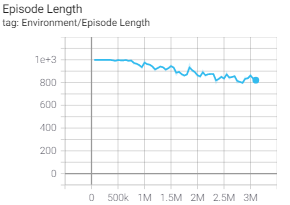
\includegraphics[width=\textwidth]{ep_len.PNG}
        \caption{Episode Length}
        \label{fig:episode length}
    \end{subfigure}
    \begin{subfigure}[b]{0.4\textwidth}
        % \centering
        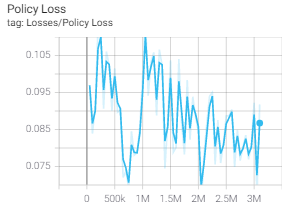
\includegraphics[width=\textwidth]{policy_loss.PNG}
        \caption{Policy Loss}
        \label{fig:policy}
    \end{subfigure}
    \begin{subfigure}[b]{0.4\textwidth}
        % \centering
        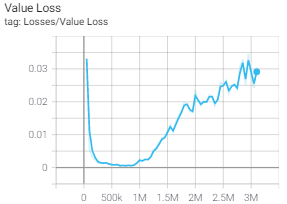
\includegraphics[width=\textwidth]{value_loss.PNG}
        \caption{Value Loss}
        \label{fig:value loss}
    \end{subfigure}
    %    \caption{Unity Enviroment Elements}
        \label{fig:unity}
\end{figure}

% \begin{figure}
% 
\includegraphics[width=0.8\linewidth]{placeholder.jpg}
% \caption{Running Curve}
% \end{figure}
% Nunc tempus venenatis facilisis. Curabitur suscipit consequat eros non porttitor. Sed a massa dolor, id ornare enim:

% \begin{table}
% \vspace{2ex}
% \begin{tabular}{l l l}
% \toprule
% \textbf{Treatments} & \textbf{Response 1} & \textbf{Response 2}\\
% \midrule
% Treatment 1 & 0.0003262 & 0.562 \\
% Treatment 2 & 0.0015681 & 0.910 \\
% Treatment 3 & 0.0009271 & 0.296 \\
% \bottomrule
% \end{tabular}
% \caption{Table caption}
% \end{table}

\end{block}

%----------------------------------------------------------------------------------------

\end{column} % End of column 2.2

\end{columns} % End of the split of column 2

\end{column} % End of the second column

\begin{column}{\sepwid}\end{column} % Empty spacer column

\begin{column}{\onecolwid} % The third column

%----------------------------------------------------------------------------------------
%	CONCLUSION
%----------------------------------------------------------------------------------------

\begin{block}{Conclusion}

So far, this project shows that given a rule set of reward and penalty, RL algorithms could work well on car self-driving tasks, no matter how the environment is. And we hope this could be a base for future self-driving cars coming into real life and even VR+AI driving school in the Hong Kong market.

\end{block}

%----------------------------------------------------------------------------------------
%	ADDITIONAL INFORMATION
%----------------------------------------------------------------------------------------
\begin{block}{Furtherwork}
Up to now, due to time and computational resource limitations, this project has several shortcomings that can be improved:
\begin{itemize}
\item Because we need more than 2 days to train a single test, so we don't have enough time to train various RL algorithms and make further comparisons(PPO was done, but SAC is still in progress).
\item There is only one agent(i.e., the car) in the driving environment. In the future, we hope to add more agents to co-operate in the simulated world. For example, at present, all the red balls are defined by a uniform random function, which we hope can replace by pedestrian agents.
\item As for environmental construction, we think we can do more exquisitely to be closer to the real-world layout.
\end{itemize}

\end{block}

%----------------------------------------------------------------------------------------
%	REFERENCES
%----------------------------------------------------------------------------------------

% \begin{block}{References}

% \nocite{*} % Insert publications even if they are not cited in the poster
% \small{\bibliographystyle{unsrt}
% \bibliography{sample}\vspace{0.75in}}

% \end{block}

%----------------------------------------------------------------------------------------
%	ACKNOWLEDGEMENTS
%----------------------------------------------------------------------------------------

\setbeamercolor{block title}{fg=red,bg=white} % Change the block title color

\begin{block}{Video Demo}

\small{\rmfamily{Here are some running captured during our experiments \\ \href{run:./demo.mkv}{Click to Open Car Demo}}} \\
 
\ 

\begin{figure}[bH]
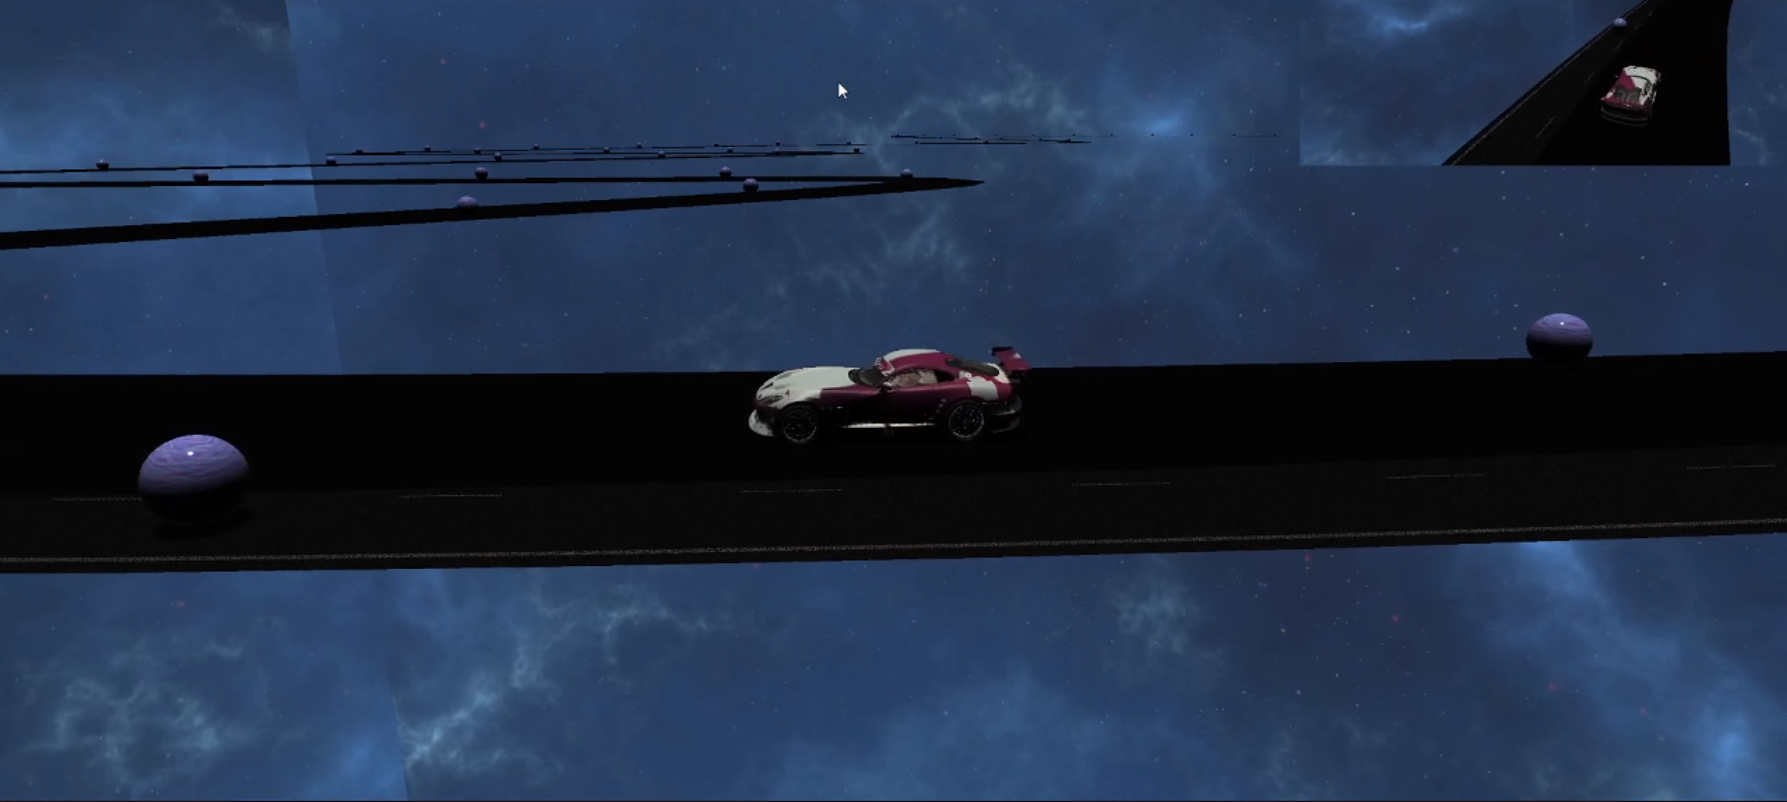
\includegraphics[width=\textwidth]{running.png}
\end{figure}

\end{block}

%----------------------------------------------------------------------------------------
%	CONTACT INFORMATION
%----------------------------------------------------------------------------------------

% \setbeamercolor{block alerted title}{fg=black,bg=norange} % Change the alert block title colors
% \setbeamercolor{block alerted body}{fg=black,bg=white} % Change the alert block body colors

% \begin{alertblock}{Contact Information}

% \begin{itemize}
% \item Web: \href{http://www.university.edu/smithlab}{http://www.university.edu/smithlab}
% \item Email: \href{mailto:john@smith.com}{john@smith.com}
% \item Phone: +1 (000) 111 1111
% \end{itemize}

% \end{alertblock}

% \begin{figure}[bH]
% 
\includegraphics[width=0.4\linewidth]{logo.png}
% \end{figure}

%----------------------------------------------------------------------------------------

\end{column} % End of the third column

\end{columns} % End of all the columns in the poster

\end{frame} % End of the enclosing frame

\end{document}